%%%%%%%%%%%%%%%%%%%%%%%%%%%%%%%
%%% 第二章 基于深度学习的机械臂分拣系统设计
%%%%%%%%%%%%%%%%%%%%%%%%%%%%%%%

\chapter{基于深度学习的机械臂自动分拣系统设计}

自动分拣系统的核心为图像处理模块,该模块的核心为目标检测算法。传统的目标检测算法需要人为为工件构造特征,
通过模板匹配的方式确定工件位置,再通过分类器的方式确定工件类别。当变换检测工件时,就需要针对工件再次构造特征。
而基于深度学习的目标检测算法则可以实现端到端的训练。这使得基于深度学习的机械臂分拣系统具有很强的可移植性。

自动分拣系统是一个多模块协同作用的系统。包括图像采集模块、图像处理模块和机械臂控制模块。这三个模块均建立在硬件
基础之上,且需要高效的通信机制。本章主要介绍整个自动分拣系统的整体架构和底层设计,包括硬件选型、通信流程等。然后
介绍了如何选择本系统中使用的目标检测算法,至于具体模型的介绍、训练及部署等,将放到第三章去讨论。最后,本章将介绍
目前相对已经比较成熟的手眼标定及机械臂控制方法。

\section{系统整体架构}

系统的逻辑层面的架构图如图    \ref{fig:total_construct}
所示。

\begin{figure}[htbp]
    \centering
    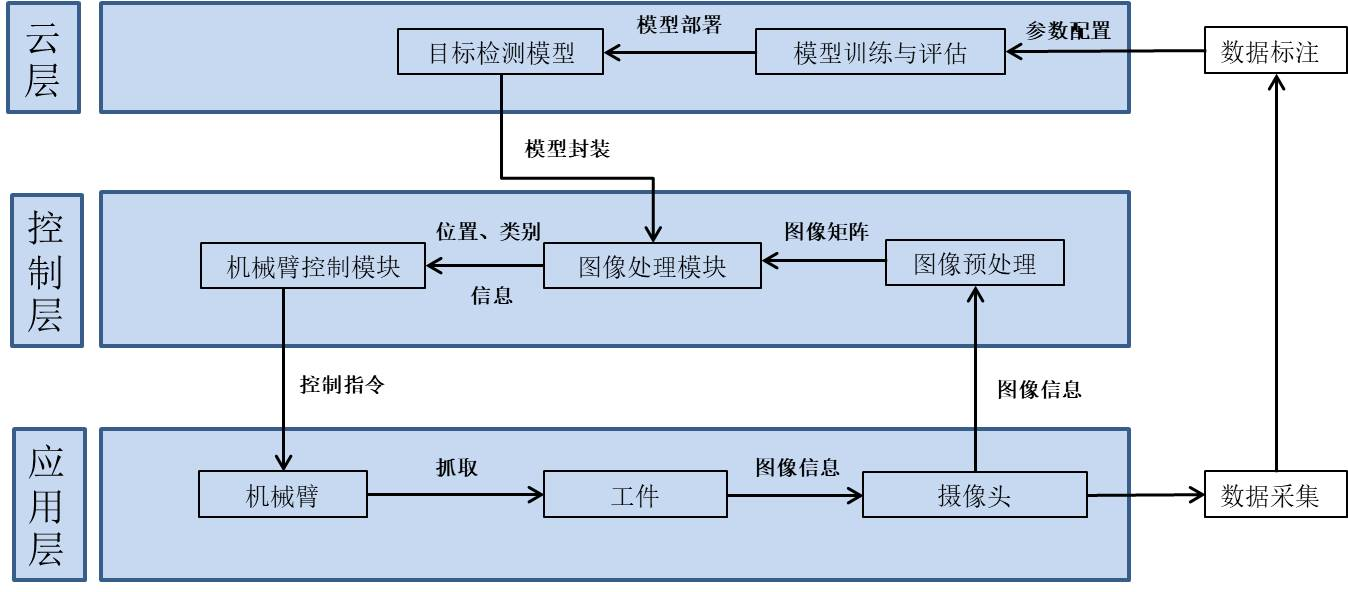
\includegraphics[width=\textwidth]{pic/chap2/total_construct.jpg}
    \caption{系统逻辑架构图}
    \label{fig:total_construct}
\end{figure}

基于深度学习的机械臂分拣系统逻辑上可以分为三个层面:应用层、控制层和云层(即服务器层)。以下对每个层面进行具体介绍:

1. 应用层

应用层由机械臂、工件和摄像头组成。主要是摄像头收集工件信息,机械臂对工件执行抓取动作。这一层面是整个系统对外展示的层面,
代表了整个系统的表现。

2. 控制层

控制层主要进行信息的处理和机械臂的控制指令生成。首先,控制层接收由应用层摄像头发送的图像信息,并进行预处理,之后发送给图像处理
模块中的目标检测模型进行预测,得到工件的位置和类别信息,然后发送给机械臂控制模块,由机械臂控制模块生成相应的机械臂控制指令,发送给
机械臂进行执行。

其中,摄像头和控制层的通信通过USB完成,所使用的摄像头为USB摄像头,主要是进行图像信息的传输;控制层和机械臂之间通过串口进行通信,
主要是进行机械臂控制指令的传输,如G代码等;而控制层的模块之间,则通过
机器人控制系统(Robot Operation System,ROS)进行,主要进行整型或浮点数的传输。

3. 云层(服务器层)

服务器层主要用于系统的搭建,在系统运行时是不参与工作的。服务器主要提供计算资源,用于深度学习模型的训练和评估。训练完成后,得到的其实是模型配置文件
和由大量浮点数组成的权重文件。模型配置文件主要用于描述模型的结构和参数,权重文件则用于描述模型网络的各个参数值。有了这些,就可以将模型部署和封装到
控制层,用于预测图像中工件的位置和信息。

此外,在三个层之外,还需要使用摄像头采集数据集,并进行标注,用作服务器层模型训练的数据集。

\section{系统硬件选型}

作为机械自动化及高性能计算一体的系统,基于深度学习的自动化分拣系统对硬件环境非常依赖。硬件性能的好坏将直接影响目标检测模型
的迭代次数、机械臂响应速度和分拣的延迟。因此,自动分拣系统的硬件选型非常重要。

本节主要介绍系统的硬件选型,包括用于采集图像信息的USB摄像头、用于高性能计算的服务器、运行图像处理模块和机械臂控制模块的
高性能嵌入式平台以及用于抓取工件的机械臂。

\subsection{目标检测模型训练用服务器}

深度学习模型的训练需要大量的计算资源,由于大量参数的反向传播计算需要大规模的矩阵运算能力,因此,模型训练用服务器需要配备
GPU,用来加速训练。同时,其CPU性能和IO性能也有一定要求,以支撑大量图像文件的处理。基于以上要求,本文配备的服务器软硬件环境如
表\ref{table:server:config}所示。实体图如图 \ref{fig:server} 所示。

{
    \begin{table}[htb] 
        \zihao{5}
        \caption{服务器软硬件环境详情表}
        \label{table:server:config}
        \centering
        \begin{tabular}[t]{c|c|c|c}
            \hline
            名称 & 配置  & 名称 & 配置\\
            \hline
            型号 & 戴尔 T630 & 操作系统 & Ubuntu 14.04.5 \\
            \hline
            CPU & DDR4 16G*8 & 数据库 & SQLite\\
            \hline
            SSD & 512G & 编译环境 & C++/Python3.6.5/CUDA9.0/Cudnn5\\
            \hline
            硬盘 & 4T SAS 7.2K*1 & 网络带宽 & 按固定带宽(6MPS)\\
            \hline 
            GPU & NVIDIA GTX1080Ti*2 & 其他服务 & Anconda/JupyterHub\\
            \hline
            电源 & 双电源1100W*2 & & \\
            \hline
        \end{tabular} 
    \end{table}
}

\begin{figure}[h]
    \centering
    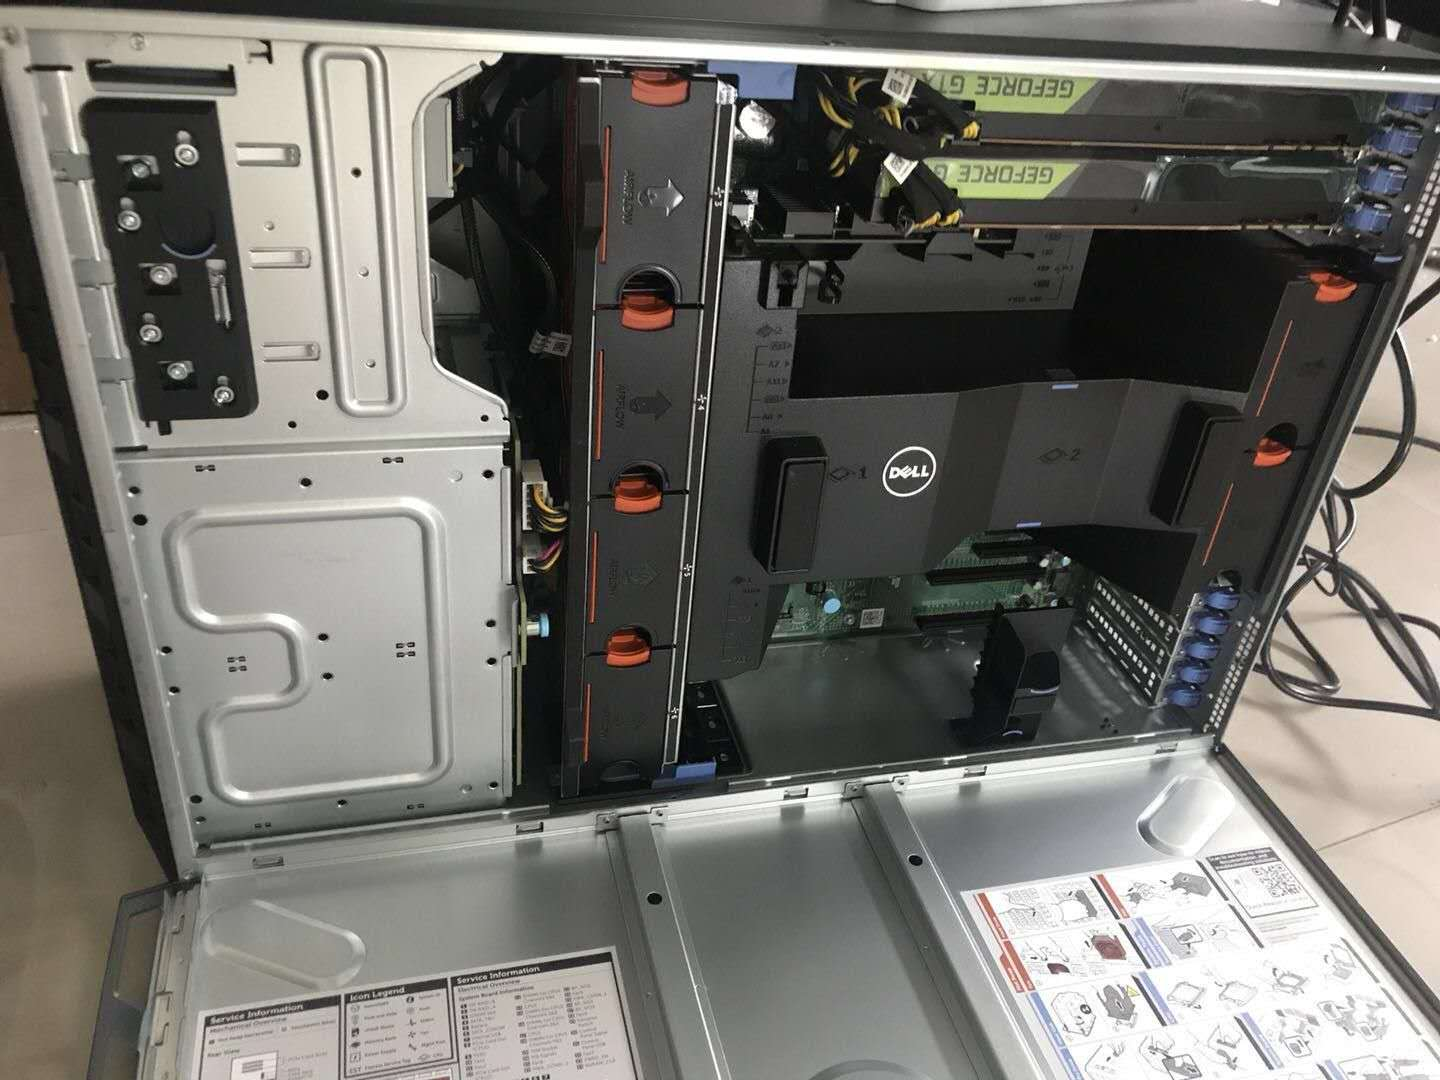
\includegraphics[width=0.6\textwidth]{pic/chap2/server.jpg}
    \caption{服务器实体图}
    \label{fig:server}
\end{figure}

本文选用的GPU型号为NVIDIA GTX1080Ti。GPU为图形处理器的简称,图形处理器是英伟达公司首先提出的概念。GPU不同于传统的CPU,其内核数量众多,一般
拥有数百或数千个内核,经过优化可运行大量计算,对深度学习算法尤其有用。GPU在深度学习计算上,比传统CPU运行相同计算速度快10~100倍。使用GPU训练深度学习
模型十分快速,能够帮助我们快速迭代模型,快速找到最优参数。

\subsection{目标检测运行硬件平台} 

基于深度学习目标检测模型的自动分拣系统,其核心图像处理模块需要具备较强的运算能力,来执行深度学习模型的预测功能。传统的自动分拣系统,一般使用高性能台式主机
作为图像处理模块的运行硬件平台,但对于基于深度学习目标检测模型的自动分拣系统来说,图像处理模块需要运行在配备GPU的硬件平台上,而若使用配备GPU的台式主机,
一是成本高昂、二是体积大,不便搬运。因此,本文使用NVIDI研发的Jetson TX2 \cite{TX2} 作为图像处理模块的运行平台。

Jetson TX2是一台模块化的人工智能超级计算机,采用NVIDIA Pascal架构。其性能强大,外形小巧,节能高效,非常适合机器人、无人机、智能便携式设备等
场景。简单来说,Jetson TX2是一款具备GPU运算能力的嵌入式单元,其大小与普通嵌入式设备的处理器类似,但计算能力远超后者。其外观如图 \ref{fig:jetson_tx2} 所示。
使用Jetson TX2,自动分拣
系统可以具备使用深度学习进行预测的能力,并且大大减少了整个系统的体积,只需要一个机械臂占用的空间即可完成整个自动分拣功能。
这使得自动分拣系统不仅仅能够在静止状态下进行分拣,同时可以进行功能扩展,在运动过程中进行分拣。同时,小巧的体积能够增加自动分拣系统机械臂
的密度,有效处理工件密集时机械臂数量不足的问题。总之,本文将Jetson TX2应用于分拣系统中,不仅能够完成自动分拣功能,并且大大扩展了自动分拣系统
的功能,使得其应用场景更加广泛。

\begin{figure}[h]
    \centering
    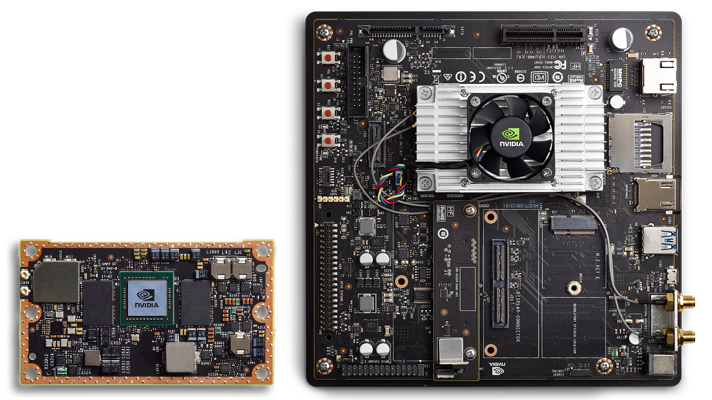
\includegraphics[width=\textwidth]{pic/chap2/jetson_tx2.jpg}
    \caption{Jetson TX2示意图}
    \label{fig:jetson_tx2}
\end{figure}

本文使用的Jetson TX2硬件规格如表 \ref{table:TX2:config} 所示。

{
    \begin{table}[htb] 
        \zihao{5}
        \caption{Jetson TX2硬件环境详情表}
        \label{table:TX2:config}
        \centering
        \begin{tabular}[t]{c|c}
            \hline
            名称 & 配置  \\
            \hline
            GPU & NVIDIA Pascal, 256 CUDA cores  \\
            \hline
            CPU & HMP Dual Denver 2/2 MB L2+ \& Quad ARM A57/2 MB L2 \\
            \hline
            内存 & 8GB 128 bit LPDDR4 59.7GB/s\\
            \hline
            CSI & CSI2 D-PHY 1.2\\
            \hline 
            硬盘存储 & 32GB eMMC, SDIO, SATA\\
            \hline
            USB & USB 3.0 + USB 2.0 \\
            \hline
        \end{tabular} 
    \end{table}
}

Jetson TX2的软件环境由JetPack构建。NVIDIA JetPack SDK 是用于构建Jetson TX2人工智能应用最全面的解决方案。使用JetPack可以为
Jetson TX2安装操作系统、高性能计算库和开发工具。本文采用JetPack 4.1.1为Jetson TX2进行刷机,最终构建的软件环境如表\ref{table:TX2:software}所示。

{
    \begin{table}[htb] 
        \zihao{5}
        \caption{Jetson TX2软件环境详情表}
        \label{table:TX2:software}
        \centering
        \begin{tabular}[t]{c|c}
            \hline
            名称 & 介绍  \\
            \hline
            操作系统 & Linux tegra-ubuntu 4.4.15-tegra\\
            \hline
            TensorRT & 高性能深度学习推理库,加速深度学习推理,\\
             & 减少卷积神经网络运行时的内存占用  \\
            \hline
            CUDA & 为深度学习框架提供加速API \\
            \hline
            OpenCV & 用于图像处理和计算机视觉的开源库\\
            \hline
            cuDNN & 深层神经网络的GPU加速库\\
            \hline 
            VisionWorks & 计算机视觉和图像处理的软件开发包\\
            \hline
        \end{tabular} 
    \end{table}
}

在实际使用过程中,Jetson TX2有多种模式,其工作模式及相应的CPU和GPU频率如表\ref{table:TX2:mode}所示。Jetson TX2在使用时默认最低功耗模式1,风扇不转。
应用在自动分拣系统中,结合深度学习目标检测算法高计算量的实际情况,在实际使用中,我们使用其最大功耗模式,来获得最高的计算性能。直接运行sudo sh jetson\_clocks.sh开启最大功耗模式。


{
    \begin{table}[htb] 
        \zihao{5}
        \caption{Jetson TX2各工作模式介绍}
        \label{table:TX2:mode}
        \centering
        \begin{tabular}[t]{c|c|c|c|c|c|c}
            \hline
            Mode & mode Name & Denver 2 & CPU频率 & ARM A57 & Frequency & GPU频率  \\
            \hline
            0 & Max-N & 2 & 2.0GHZ & 4 & 2.0GHZ & 1.30GHZ \\
            \hline 
            1 & Max-Q & 0 & & 4 & 1.2GHZ & 0.85GHZ \\
            \hline
            2 & Max-P Core-All & 2 & 1.4GHZ & 4 & 1.4GHZ & 1.12GHZ \\
            \hline
            3 & Max-P ARM & 0 & & 4 & 2.0GHZ & 1.12GHZ \\
            \hline
            4 & Max-P Denver & 2 & 2.0GHZ & 0 & & 1.12GHZ \\
            \hline
        \end{tabular} 
    \end{table}
}

Jetson TX2是自动分拣系统的“大脑”,自动分拣系统的图像处理模块和机械臂控制模块均运行在该嵌入式硬件平台之上。Jetson TX2接收
USB端口发来的图像信息,经过处理后,转化为机械臂的控制G代码,通过串口发送给机械臂执行微机,控制机械臂执行抓取动作。


\subsection{摄像头}

Jetson TX2支持的摄像头有USB摄像头和CSI摄像头。其优缺点对比如表\ref{table:camera:compare}所示 \cite{CSI}。

{
    \begin{table}[htb] 
        \zihao{5}
        \caption{CSI和USB摄像头对比}
        \label{table:camera:compare}
        \centering
        \begin{tabular}[t]{c|c|c}
            \hline
             & CSI摄像头 & USB摄像头  \\
            \hline
            优点 & 根据CPI和内存进行优化; & 易整合; \\
                & 充分利用视觉管线; & 可以做很多离线的图像工作;\\
                & 可底层访问摄像头。 & 可长距离工作,支持大图像传感器。 \\
            \hline 
            缺点 & 支持距离过短; & 占用CPU;\\
                 & 价格昂贵。 & 对于硬件编码支持不良。\\
            \hline
        \end{tabular} 
    \end{table}
}

相比于CSI摄像头,USB摄像头具有工作距离长,成本低、与Jetson TX2松耦合的特点,因为本文选用USB摄像头作为图像采集
设备。同时,图像采集设备与Jetson TX2的通信采用USB完成。如图\ref{fig:USB_camera},最终选择罗技C270款USB摄像头作为图像采集设备。
设定采集图像尺寸为640*480。用于采集图像的工件为实验室3D打印件。为了用于本文实验,使用3D打印机打印出两个打印体
作为工件,其形状如图\ref{fig:printer}所示。图中两个工件的代号从上到下依次为fo和dabai。

\begin{figure}[h]
    \begin{minipage}[t]{0.45\textwidth}
        \centering
        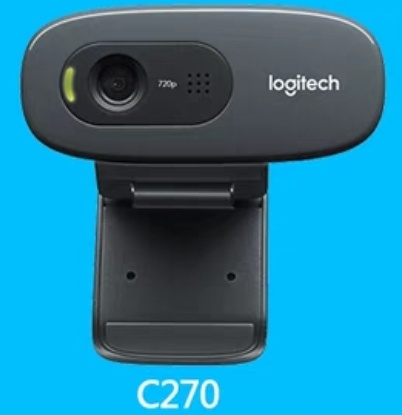
\includegraphics[width=0.8\textwidth]{pic/chap2/USB_camera.jpg}
        \caption{图像采集设备: USB摄像头}
        \label{fig:USB_camera}
    \end{minipage}
    \begin{minipage}[t]{0.45\textwidth}
        \centering
        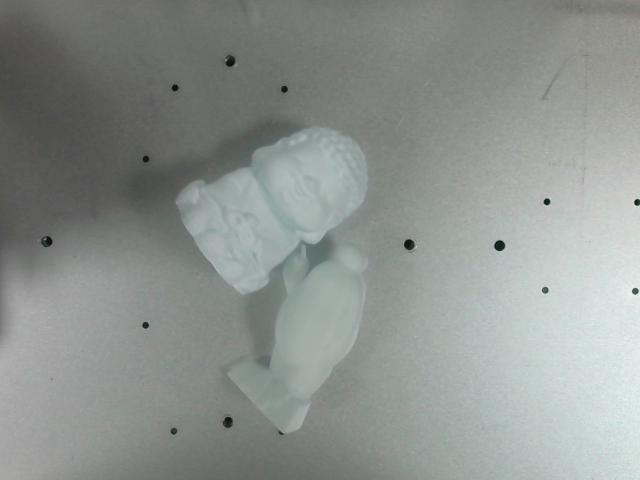
\includegraphics[width=0.8\textwidth]{pic/chap2/printer.jpg}
        \caption{3D打印工件替代品}
        \label{fig:printer}
    \end{minipage}
\end{figure}

\subsection{机械臂选型}

结合成本及使用便利性等基本情况,本文采用的机械臂为越疆DOBOT魔术师系列轻量型机械臂。该系列机械臂适用于多种
应用场景,可根据需求增删模块,从而实现不同功能。使用该机械臂能降低自动分拣系统的各个模块之间的耦合,便于
多模块开发与管理。该款机械臂如图\ref{fig:robot}所示。

\begin{figure}[h]
    \centering
    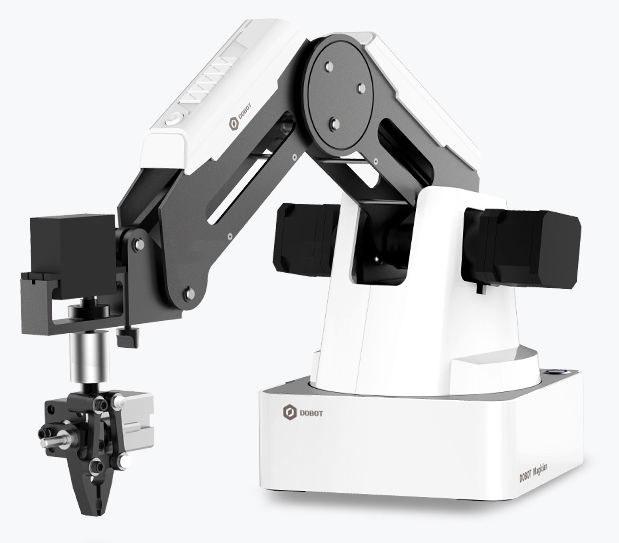
\includegraphics[width=0.6\textwidth]{pic/chap2/robot.jpg}
    \caption{机械臂示意图}
    \label{fig:robot}
\end{figure}

DOBOT提供了配套的Arduino套件和用于接收控制信号的可扩展I/O接口,可用于二次开发。具体来说,Jetson TX2处理图像
后产生的控制机械臂的G代码,通过I/O接口发送到DOBOT的Arduino套件上,Arduino根据G代码发出相应的控制信号,控制DOBOT
的各个舵机,从而产生相应的运动。

同时,为了使DOBOT适用于抓取分拣的任务场景,我们将机械臂末端模块换做定制的机械夹持器,用于抓取工件。本文设计的自动分拣系统
不考虑工件抓取姿态,因此不需要考虑工件三维信息。机械夹持器抓取时,定位到工件中心点,完全张开进行抓取。机械夹持器规格和实物
如图\ref{fig:grip} 所示。

\begin{figure}[h]
    \centering
    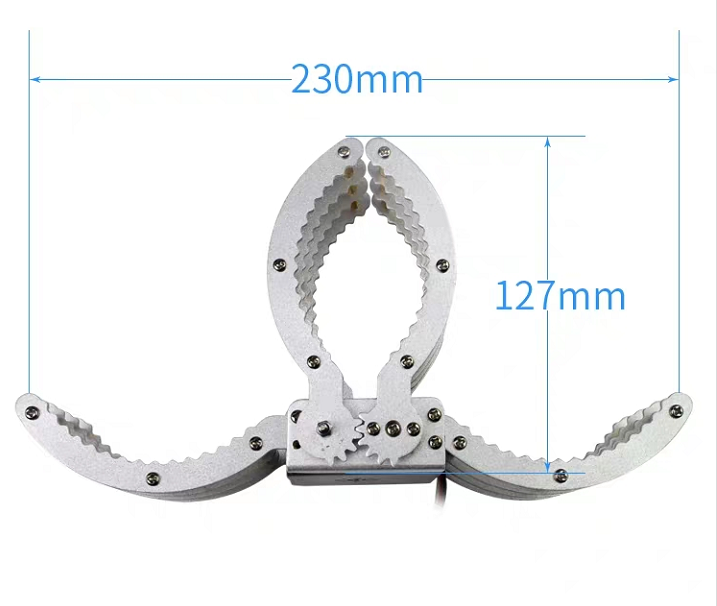
\includegraphics[width=0.6\textwidth]{pic/chap2/grip.png}
    \caption{机械夹持器示意图}
    \label{fig:grip}
\end{figure}


\subsection{系统硬件架构}

自动分拣系统的硬件架构如图 \ref{fig:hardware_construct} 所示。

\begin{figure}
    \centering
    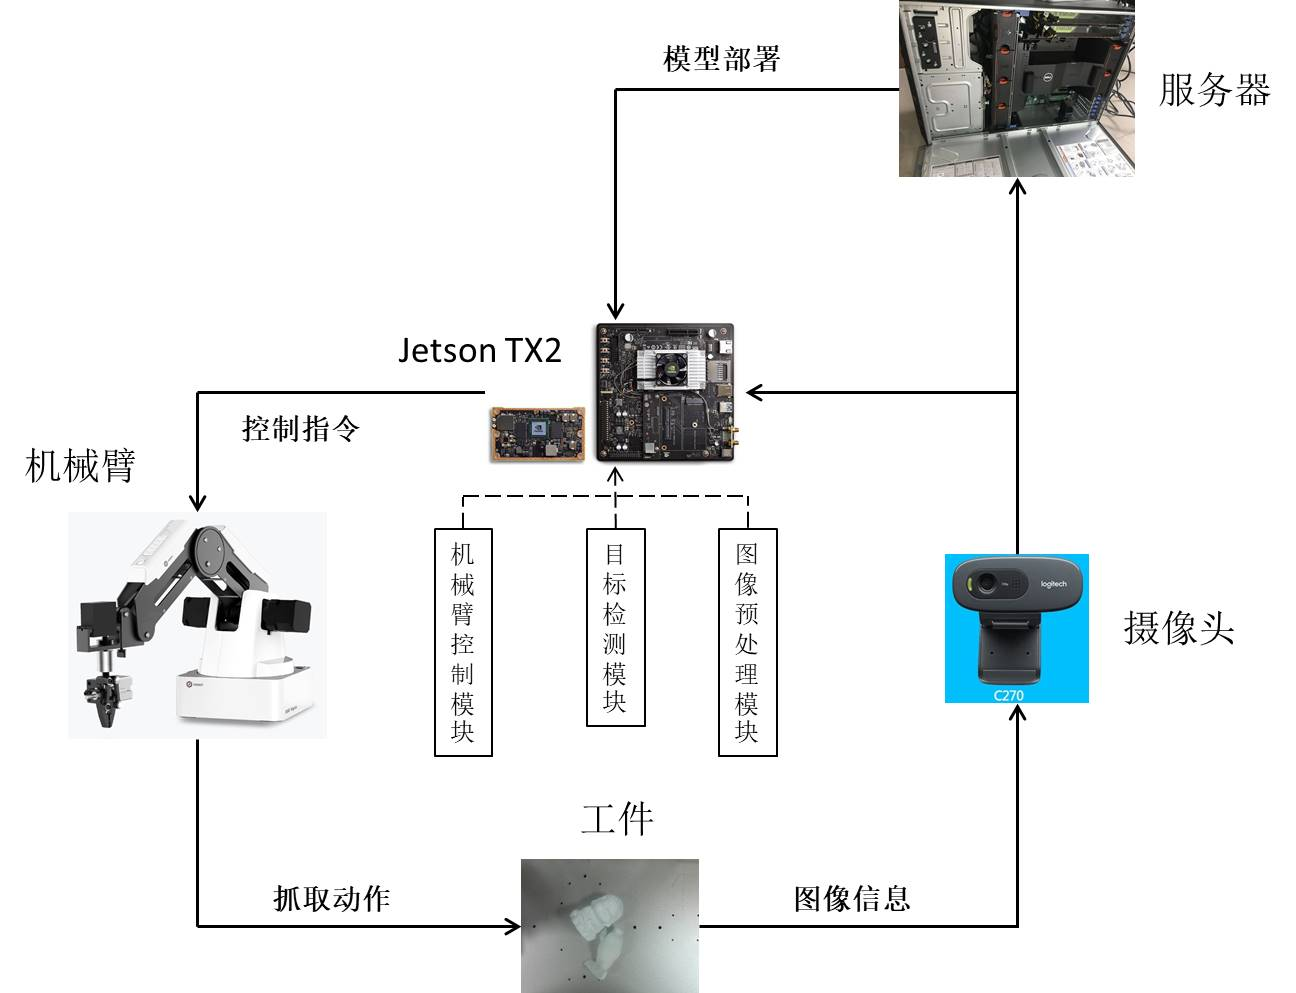
\includegraphics[width=\textwidth]{pic/chap2/hardware_construct.jpg}
    \caption{系统硬件架构图}
    \label{fig:hardware_construct}
\end{figure}

USB摄像头采集工件图像信息,通过USB传输方式将图片传递给Jetson TX2。图片首先传递给Jetson TX2上的图像预处理模块,处理后
发送给Jetson TX2上的目标检测模块,获取工件位置和类别信息后发送给Jetson TX2上的机械臂控制模块,机械臂控制模块生成G代码控制
指令之后。Jetson TX2上各模块之间的通信通过ROS话题通信机制完成。随后,机械臂控制模块通过串口发送给机械臂中的Arduino套件,
然后控制舵机生成机械臂运动轨迹,对工件进行抓取。Jetson TX2和机械臂之间通过串口进行通信。整个数据和执行流程以工件为连接形成
一条回路。

\section{系统模块间通信机制}

自动分拣系统由多个硬件模块协同完成,硬件之间的通信不可避免。同时,Jetson TX2上运行着自动分拣系统的多个软件模块,该嵌入式
平台内部也需要一定的通信机制来完成软件模块之间的通信。本小节将基于不同的硬件和应用场景选择合适的通信方法。

\subsection{USB通信}

自动分拣系统的核心是目标检测算法。而目标检测算法需要图像作为输入,因此需要使用摄像头获取图像信息。摄像头需要将图像信息传递给
运行目标检测算法的Jetson TX2。因此需要摄像头和Jetson TX2之间的通信。双设备通信方法一般有USB和蓝牙、WIFI等通信方法。
其中USB为有线通信方式,蓝牙和WIFI为无线通信方式。有线传输速度高于无线传输,但不适用于长距离和经常变动位置的设备通信。
而摄像头、Jetson TX2和机械臂三个硬件的位置相对固定,因此采用有线传输进行通信。

本系统中,USB通信主要用于摄像头向Jetson TX2传递图像信息。
本课题使用的USB版本为USB 3.0    \cite{USB3.0}版本,其传输速度为5Gbit/s,足以支撑高FPS的图像传输。

\subsection{ROS通信}

自动分拣系统的硬件核心为Jetson TX2,其上运行着图象预处理模块、图像处理(目标检测)模块和机械臂控制模块三部分。三个模块之间需要
进行实时数据传输,以完成自动分拣。Jetson TX2上的三个模块可看做Linux系统下的三个进程,而进程间的通信方式有管道、信号、消息队列、
共享内存和套接口等。\cite{jincheng_comm}但以上方法过于底层,实现复杂、效率低下。

ROS(Robot Operation System)\cite{ROS}是一个机器人分布式框架。ROS基于Linux系统的OS层,实现了高封装特性的ROS通信库,可以在
ROS各节点之间实现异步通信。其架构如图\ref{fig:ROS_construct}所示\cite{ROS_book}。

\begin{figure}[h]
    \centering
    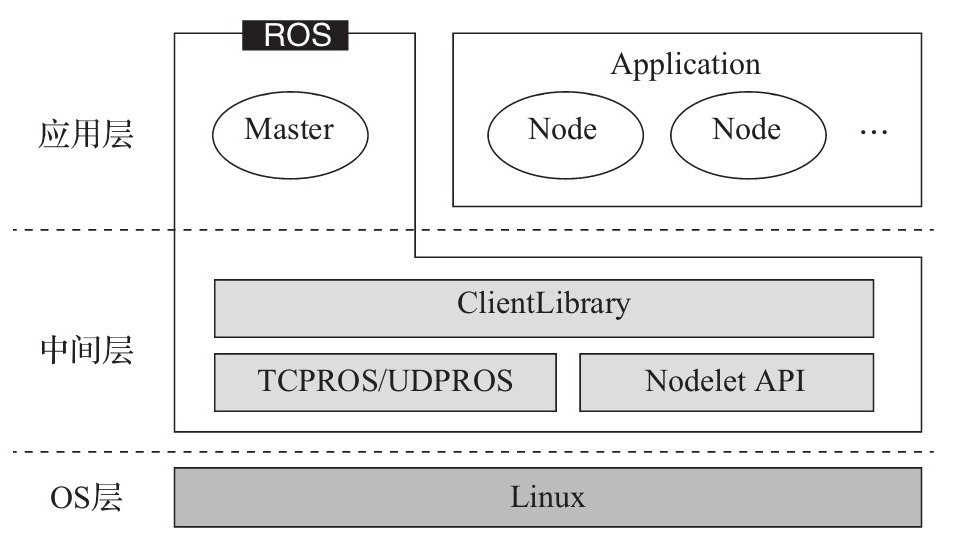
\includegraphics[width=\textwidth]{pic/chap2/ROS_construct.jpg}
    \caption{ROS架构图}
    \label{fig:ROS_construct}
\end{figure}

ROS提供了基于TCP/UDP网络的通信系统,使用发布/订阅、客户端/服务端等模型,实现多种通信机制的数据传输。ROS系统的功能模块以节点为单位独立
运行,可以分布于多个相同或不同的主机上,在系统运行时以端对端的拓扑结构进行连接。同时,ROS可以使用一个
管理者-Master管理整个系统的运行。因此自动分拣系统中,Jetson TX2上运行的三个模块可以分别作为ROS中的三个节点运行,
使用ROS的Master节点进行统一管理和通信。

本文使用ROS话题通信机制进行Jetson TX2上各程序模块之间的通信。
话题通信机制采用发布/订阅的通信模型。假定Talker为发布消息的ROS节点,Listener为订阅该消息的ROS节点,则该通信模型的通信步骤如下:
\begin{enumerate}
    \item{Talker注册。Talker启动后,使用RPC向ROS Master注册发布者信息,包括发布消息的话题名;ROS Master将节点的注册信息加入注册列表。}
    \item{Listener注册。Listener启动后,同样通过RPC向ROS Master注册订阅者信息,包括需要订阅的话题名。}
    \item{ROS Master进行匹配。Master根据Listener的订阅信息从注册列表中进行查找,若未找到,则等待发布者的发布;若找到匹配
    的发布者信息,则通过RPC向Listener发送Talker的RPC地址信息。}
    \item{Listener发送连接请求。Listener收到Talker的地址信息后,尝试通过RPC向Talker发送连接请求。}
    \item {Talker确认连接请求。Talker收到Listener的连接请求后,继续通过RPC向Listener确认连接信息,其中包括自身的TCP地址信息。}
    \item {Listener与Talker建立网络连接。Listener接收到确认信息后,通过收到的TCP地址信息与Talker建立网络连接。}
    \item {Talker向Listener发送消息。建立连接后,Talker将数据发送到Listener节点。}
\end{enumerate}

在自动分拣系统中的Jetson TX2硬件模块中,我们使用ROS进行其上运行的软件模块的管理和通信。具体来说,在Jetson TX2中建立ROS
系统,创造usb\_camera节点,用于接收摄像头图像信息并发布图像话题消息;创造image\_preprocess节点,用于接收usb\_camera节点发布
的消息,并将图象预处理后的结果进行发布;创造yolov3节点,用于接收usb\_camera节点发布的图像消息,输入目标检测模型进行预测,将边框和
类别消息进行发布;创造robot\_control节点,用于接收yolov3节点的消息,根据图像中工件的边框和类别消息生成控制机械臂的G代码,通过串口
发送到机械臂进行执行。Jetson TX2上通过ROS进行通信的网络节点拓扑关系如图\ref{fig:ROS_com}所示。

\begin{figure}
    \centering
    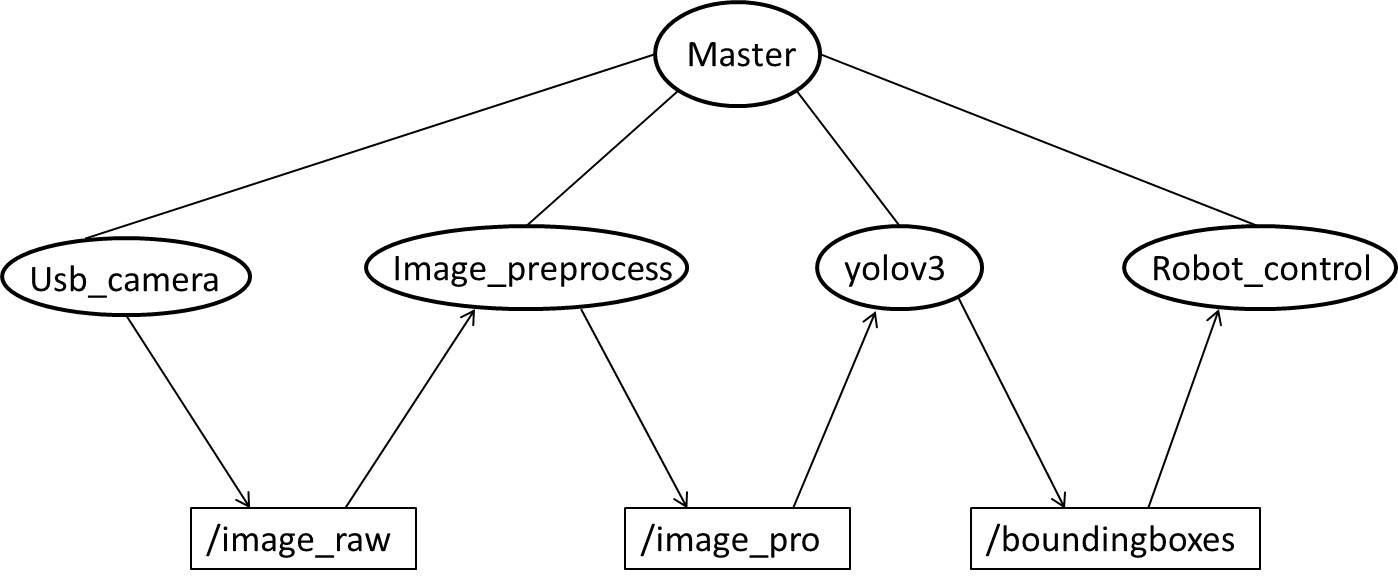
\includegraphics[width=\textwidth]{pic/chap2/ROS_com.jpg}
    \caption{Jetson TX2上的ROS通信网络图}
    \label{fig:ROS_com}
\end{figure}

其中,椭圆形节点为ROS中的节点,所有节点通过Master节点进行中转连接。方框形节点为ROS节点发布的话题名。椭圆形节点指向方框形节点
代表该节点发布了该话题;方框形节点指向椭圆形节点代表该话题被该节点所订阅。每个话题均需要设计对应的数据传输类型和结构。/image\_raw
话题用于传递摄像头采集的原始图像信息,其类型为sensor\_msgs/Images,代表传感器数据类型中的图片类型。/image\_pro为Image\_preprocess节点
经过预处理后的图像消息,其类型依然为sensor\_msgs/Images,该节点主要用于过滤无用图像消息,即无需进行抓取的图片。/boundingboxes为
yolov3节点发布的消息,yolov3节点接收图片输入,经目标检测模型预测,输出图片中工件的位置和类别信息;其类型为自定义话题消息类型,包含
类别、置信度和边框信息。各话题消息具体结构及描述如表\ref{table:ROS:node_topic}所示。

表\ref{table:ROS:node_topic}中,sensor\_msgs/Images使用数组描述图片,以一维数组存储所有像素点的RGB像素值。自定义话题消息用于描述
工件类别和边框信息。其中Class和probability描述类别及其置信度信息,其结果可能为多个,可用于后续根据置信度选择使用哪个类别;x和y用于描述
边框信息,xmin和xmax分别表示矩形边框的最小和最大横坐标,ymin和ymax分别表示矩形边框的最小和最大横坐标,其取值范围不超过图片的宽度和高度。


{
    \begin{table}[htb] 
        \zihao{5}
        \caption{Jetson TX2中各模块ROS节点发布话题描述}
        \label{table:ROS:node_topic}
        \centering
        \begin{tabular}[t]{l|l|l|l}
            \hline
            名称 & 类型 & 类型结构 & 描述  \\
            \hline
            /image\_raw & sensor\_msgs/Images & Header header  \quad    \# topic Header              & ROS自带传感器 \\
                       &                    & uint32 height  \quad    \# image height                & 类型图像消息 \\
                       &                    & uint32 width   \quad    \# image width\\
                       &                    & string encoding \quad   \# encoding of pixels\\
                       &                    & uint32 step     \quad   \# full row length in bytes \\
                       &                    & uint8[] data    \quad   \# actual matrix data \\
            \hline 
            /image\_pro  & sensor\_msgs/Images & Header header \quad     \# topic Header              & ROS自带传感器\\
                        &                    & uint32 height   \quad   \# image height                & 类型图像消息 \\
                        &                    & uint32 width     \quad  \# image width\\
                        &                    & string encoding  \quad  \# encoding of pixels\\
                        &                    & uint32 step      \quad  \# full row length in bytes\\
                        &                    & uint8[] data      \quad \# actual matrix data\\
            \hline
            /boundingboxes & 自定义话题类型 & Header header         \quad  \# topic header    & 描述工件在图片中\\
                           &               & Header image\_header  \quad  \# image header    & 的位置和类别信息\\
                           &               & string Class          \quad  \# Object category\\
                           &               & float probability     \quad  \# Classification confidence\\
                           &               & uint32 xmin           \quad  \# boundingbox min x\\
                           &               & uint32 xmax           \quad \# boundingbox max x\\
                           &               & uint32 ymin           \quad  \# boundingbox min y\\
                           &               & uint32 ymax           \quad  \# boundingbox max x       \\    
            \hline
        \end{tabular} 
    \end{table}
}


\subsection{串口通信}

DOBOT机械臂内置Arduino mega 2560控制器,因此,Jetson TX2与机械臂的通信即Jetson TX2与Arduino的通信。DOBOT控制器
提供了USB与蓝牙两种通信方式,分别对应于Arduino mega 2560的两个串口。Jetson TX2需要通过USB转串口与Arduino控制器进行
通信,即两个硬件的通信方式为特定的串口通信协议。其详细参数如表\ref{table:serial:parameter}所示。

{
    \begin{table}[htb] 
        \zihao{5}
        \caption{DOBOT串口通信协议参数说明}
        \label{table:serial:parameter}
        \centering
        \begin{tabular}[t]{c|c}
            \hline
            详细参数 & 参数说明  \\
            \hline
            波特率   & 115200bps \\
            \hline 
            数据位   & 8位 \\
            \hline
            停止位   & 1位 \\
            \hline
            校验位   & 无 \\
            \hline
        \end{tabular} 
    \end{table}
}

本文使用串口通信发送的数据为G代码指令。为了使DOBOT的Arduino支持G代码指令,我们将Marlin固件\cite{Marlin}烧入DOBOT的Arduino控制板中。
自动分拣系统使用的G-Code指令如表\ref{table:G-code:introduction}所示。

{
    \begin{table}[htb] 
        \zihao{5}
        \caption{自动分拣系统使用的G-Code}
        \label{table:G-code:introduction}
        \centering
        \begin{tabular}[t]{c|c}
            \hline
            字母 & 意义  \\
            \hline
            G   & 标准G-Code命令,例如移动到一个坐标点 \\
            \hline 
            X   & X坐标,通常用于移动命令 \\
            \hline
            Y   & Y坐标,通常用于移动命令 \\
            \hline
            Z   & Z坐标,通常用于移动命令 \\
            \hline
            A   & 自定义,用于机械臂末端夹具舵机的控制命令\\
            \hline
            F   & 修改,机械臂末端移动速度,单位:毫米/秒 \\
            \hline
            B   & 自定义,用于机械臂模块夹具舵机的速度控制,即抓取工件的速度\\
            \hline
        \end{tabular} 
    \end{table}
}


\section{目标检测算法选型}

目标检测算法是自动分拣系统的核心。目标检测算法的预测用时将直接影响自动分拣系统的实时性,目标检测算法的准确率将直接影响自动分拣系统的分拣
准确率。传统的目标检测算法需要人为为工件构造特征,通过模板匹配的方式确定工件位置,再通过分类器的方式确定工件类别,这种方法
的优势为可理解性强,模型直观清楚,但缺陷也很致命,即准确率低,鲁棒性差,可移植性差。当变换检测工件时,就需要针对工件再次构造特征。
而基于深度学习的目标检测算法则可以实现端到端的训练,且准确率远高于传统目标检测算法。这使得基于深度学习的机械臂分拣系统具有很强的可移植性和鲁棒性
。本文设计的自动分拣系统使用基于深度学习的目标检测算法。参考1.2.1小节目标检测算法研究现状,本文进行目标检测算法选型的范围为Faster R-CNN、YOLOv1、YOLOv2、Yolov3和SSD。

Faster R-CNN是two-stage流派方法的最优算法,也是第一个实现端到端训练的深度学习目标检测算法,但其网络参数众多,且在小目标检测任务上效果不尽如人意;
YOLO系列算法和SSD则属于single-stage流派方法,将边框预测问题和类别预测问题统一到一个回归问题中,直接通过整图得到物体位置和类别预测结果。这些算法
可以实现端到端训练,YOLO系列算法的主要优势为速度,不足则是针对小目标效果差;SSD的优势为提高了对小目标物体检测的效果,缺陷为非目标的小像素干扰较大。
以上算法的比较如表\ref{table:OC:compare}所示。

{
    \begin{table}[htb] 
        \zihao{5}
        \caption{目标检测算法对比}
        \label{table:OC:compare}
        \centering
        \begin{tabular}[t]{l|l|p{3cm}|p{3cm}}
            \hline
            方法名称 & 主要思想 & 优点 & 缺点  \\
            \hline
            传统目标检测方法   & 区域选择+特征提取+分类器 & 可理解性强 & 速度慢、准确率低 \\
            \hline 
            Faster RCNN   & 端到端的目标检测 & 提速、共用特征 & 训练超参数多 \\
            \hline
            YOLO   & 检测和分类从一个输出层输出 & 提速 & 小目标效果差 \\
            \hline
            YOLOv2   & 加入深度学习优化技巧 & 提速、提高精度 & 无法使用弱监督方法 \\
            \hline
            YOLOv3   & 多尺度预测,更好的分类器 & 提速、提高精度、通用性强 & 位置精度略差、召回率低 \\
            \hline
            SSD   & 多特征层提取检测框 & 提速、提高小目标检测效果 & 易受非目标小像素点干扰 \\
            \hline
        \end{tabular} 
    \end{table}
}

针对自动分拣系统的使用场景,我们需要尽可能高的检测速度。在所有的深度学习目标检测方法中,Faster RCNN由于其two-stage思想的限制,虽然
能够实现端到端训练,但其检测速度差于single-stage的方法,因此首先排除Faster RCNN。YOLO系列算法和SSD算法在COCO\cite{COCO}数据集上的表现如
表\ref{table:COCO:compare}\cite{YOLOv3:2018}所示。

{
    \begin{table}[htb] 
        \zihao{5}
        \caption{YOLO和SSD系列算法在COCO数据集上的性能比较}
        \label{table:COCO:compare}
        \centering
        \begin{tabular}[t]{l|l|l|l|l}
            \hline
            模型 & 训练集 & 测试集 & mAP值\cite{mAP} & FPS  \\
            \hline
            SSD300   & COCO trainval & test-dev & 41.2 & 46 \\
            \hline 
            SSD500   & COCO trainval & test-dev & 46.5 & 19 \\
            \hline
            YOLOv2   & COCO trainval & test-dev & 48.1 & 40 \\
            \hline
            YOLOv3-320   & COCO trainval & test-dev & 51.5 & 45 \\
            \hline
            YOLOv3-608   & COCO trainval & test-dev & 57.9 & 20 \\
            \hline
            YOLOv3-tiny & COCO trainval & test-dev & 33.1 & 220\\
            \hline
        \end{tabular} 
    \end{table}
}

由表可知,相似mAP值的情况下,YOLOv3具有更优的速度;相似FPS的情况下,YOLOv3具有更高的mAP值。同时,SSD易受非目标
小像素点干扰的情况下,考虑到自动分拣系统所在工厂环境的灰尘等小颗粒杂质较多,SSD的可用性大打折扣。综上所述,本文的自动分拣
系统的目标检测算法使用YOLOv3目标检测算法。详细配置选择及实验将在第三章第四节中进行阐述。


\section{手眼标定及机械臂控制模块设计与实现}

目标检测模块向机械臂控制模块发送的数据为工件在图片中的位置和类别信息。位置信息决定了机械臂运动的抓取位置,类别信息决定了机械臂抓取后
的放置位置。位置信息为工件在摄像头所拍到的图片中的位置,而机械臂要抓取该工件,需要知晓该工件相对机械臂的位置。而机械臂和图像并非在
同一坐标系中,因此需要通过手眼标定来统一摄像头和机械臂的坐标系。

手眼标定即相机标定+机械臂标定。机械臂标定即将机械臂坐标系转换为世界坐标系,相机标定即把图像坐标系转换为相机坐标系再转换为世界坐标系。这样
就可以确定机械臂坐标系到图像坐标系的转换关系。在实际标定过程中,可以忽略到世界坐标系转换这个步骤,直接将摄像头坐标系转换为机械臂坐标系。

本文使用的DOBOT机械臂提供笛卡尔坐标系,该坐标系规定机械臂的地盘中心为坐标原点,且机械臂末端的位置可通过其提供的API读出。因此,只需要计算
机械臂末端在图像坐标系中的坐标。这一步的计算使用九点标定法。使用机械臂工作工件中的田字格的九个点作为标定点。标定过程如图\ref{}所示。
控制机械臂分别在九个点进行触碰,
并记录在这九个点时机械臂末端在机械臂坐标系中的坐标,使用$x_{arm_{1}}$、$x_{arm_{2}}$、...、$x_{arm_{n}}$表示这些点的横坐标,y、z坐标同理,
同时,记录这九个点在图像坐标系中的坐标,使用$x_{image_{1}}$ 、$x_{image_{2}}$ 、...、$x_{image_{n}}$表示这些点的横坐标,y、z坐标同理。
使用$P_{arm}$表示将机械臂末端在机械臂坐标系中的坐标点点集合矩阵,$P_{image}$表示机械臂末端在图像坐标系中的坐标点的集合矩阵。

%%%%%%%%%%%%%%%%%%%%%%%%%%%%%%%%%%%%%%%%%%%%%%%%%%%%%%%%%%%%%%%%%%%%%%%%%%%%%%%%%%%%% TODO:九点标定过程

获得机械臂末端在机械臂末端和图像坐标系中的坐标后,只需通过一个旋转矩阵$R$和平移矩阵$T$即可获得两个坐标系之间的转换关系。即:
$$P _ { a r m } = R \cdot P _ { i m a g e } + T$$
\begin{equation}
    \centering
    \left[ \begin{array} { l l l l } { x _ { a r m _ { 1 } } } & { x _ { a r m _ { 2 } } } & { \dots } & { x _ { a r m _ { n } } } \\ { y _ { a r m _ { 1 } } } & { y _ { a r m _ { 2 } } } & { \dots } & { y _ { a r m _ { n } } } \\ { z _ { a r m _ { 1 } } } & { z _ { a r m _ { 2 } } } & { \dots } & { z _ { a r m _ { n } } } \end{array} \right] = R \cdot \left[ \begin{array} { l l l l } { x _ { i m a g e _ { 1 } } } & { x _ { i m a g e _ { 2 } } } & { \dots } & { x _ { i m a g e _ { n } } } \\ { y _ { i m a g e _ { 1 } } } & { y _ { i m a g e _ { 2 } } } & { \dots } & { y _ { i m a g e _ { n } } } \\ { z _ { i m a g e _ { 1 } } } & { z _ { i m a g e _ { 2 } } } & { \dots } & { z _ { i m a g e _ { n } } } \end{array} \right] + T
    \label{equation:loc_trans}
\end{equation}

将$R$和$T$合并得:

\begin{equation}
    \centering
    \begin{bmatrix}  x_{arm_1} & x_{arm_2} & …& x_{arm_n} \\ 
    y_{arm_1} & y_{arm_2} & …& y_{arm_n} \\  
    z_{arm_1} & z_{arm_2} & …& z_{arm_n} \end{bmatrix} = 
    \left [ \begin{array}{c|c} \begin{matrix} R \end{matrix}& \begin{matrix} T \end{matrix} \end{array} \right ] \cdot 
    \begin{bmatrix}  x_{image_1} & x_{image_2} & …& x_{image_n} \\  y_{image_1} & y_{image_2}  & …  & y_{image_n} \\  z_{image_1} & z_{image_2}  & …  & z_{image_n}  \\ 1&1&…&1 \end{bmatrix}
    \label{equation:loc_trans2}
\end{equation}

接下来就是求图像坐标到机械臂坐标的转换关系$C_{itoa} = \left [ \begin{array}{c|c} \begin{matrix} R \end{matrix}& \begin{matrix} T \end{matrix} \end{array} \right ]$,
可以通过左边点乘${P_{image}}^{-1}$得到,即:$C_{itoa} =  P_{arm} \cdot {P_{image}}^{-1}$。

\begin{figure}[h]
    \centering
    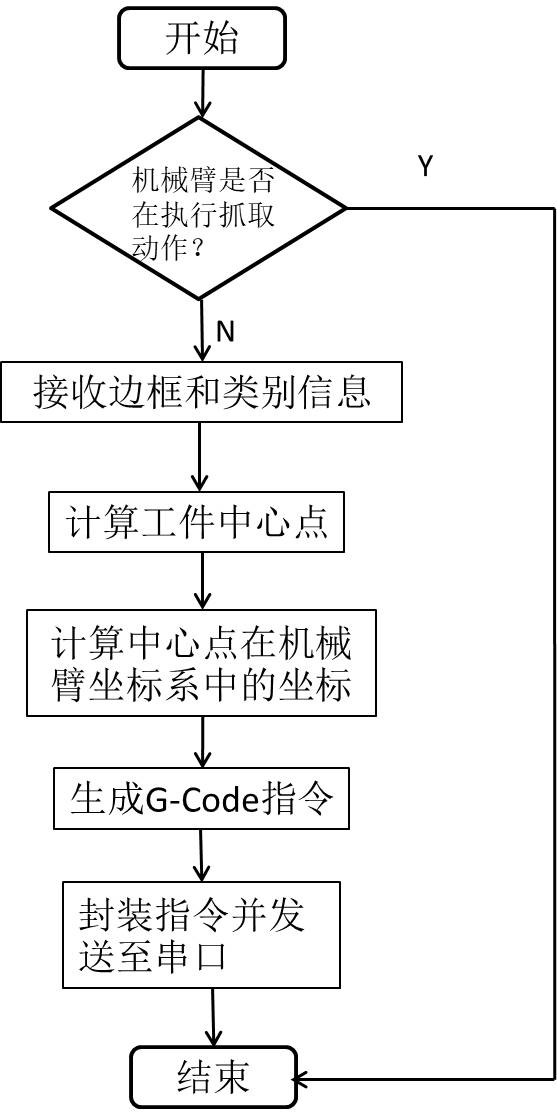
\includegraphics[scale=0.7]{pic/chap2/robot_control.jpg}
    \caption{机械臂控制模块逻辑流程图}
    \label{fig:robot:control}
\end{figure}

同理,$C_{atoi} =  P_{image} \cdot {P_{arm}}^{-1}$。

求出$C_{itoa}$之后,根据工件在图像坐标系中的坐标,即可求出工件在机械臂坐标系中的坐标。接下来只需要生成相应的G代码,控制机械臂前往目标
坐标点抓取即可。这一部分即机械臂控制模块的具体内容。机械臂控制模块的代码在一次抓取过程中的逻辑如图\ref{fig:robot:control}所示。



上图为机械臂控制模块一次正常抓取过程的逻辑流程。该模块使用cpp代码实现,通过回调函数实时监控/boundingboxes话题下的消息发布情况。每当回调
函数监控到消息方法,均执行一次以上流程。

\section{本章小结}
本章主要介绍整个自动分拣系统的整体架构和底层设计,包括硬件选型、通信流程等。然后根据各个深度学习目标检测算法的优缺点,结合具体
使用场景,进行了自动分拣系统的目标检测算法的选型,选定YOLOv3作为本文自动分拣系统的深度学习目标检测算法。最后,本章介绍了手眼标定以及
机械臂控制模块的设计与实现。

